\documentclass{standalone}
\usepackage{tikz}
\usepackage{amsmath, amssymb, latexsym}
\DeclareMathOperator{\ReLU}{ReLU}
\newcommand{\KL}{\ensuremath{\mathrm{KL}}}
\newcommand{\Ber}{\ensuremath{\mathrm{Ber}}}
 
\usepackage{tikz}
\usepackage{xcolor}

\definecolor{h}{HTML}{228B22}
\definecolor{bias}{HTML}{87CEFA}
\definecolor{conv}{HTML}{FFA500}

\definecolor{bn}{HTML}{FFD700}

\tikzset{conv/.style={black,draw=black,fill=conv,rectangle,minimum height=1cm}}
\tikzset{bn/.style={black,draw=black,fill=bn,rectangle,minimum height=1cm}}
\tikzset{rcb/.style={draw, fill=bias, minimum height=1cm}}
\tikzset{elu/.style={draw, fill=h, minimum height=1cm}}

\newcommand{\bt}{\mathbf{t}}
\newcommand{\bx}{\mathbf{x}}
\newcommand{\by}{\mathbf{y}}
\newcommand{\bz}{\mathbf{z}}
\newcommand{\eq}{=}




\begin{document}

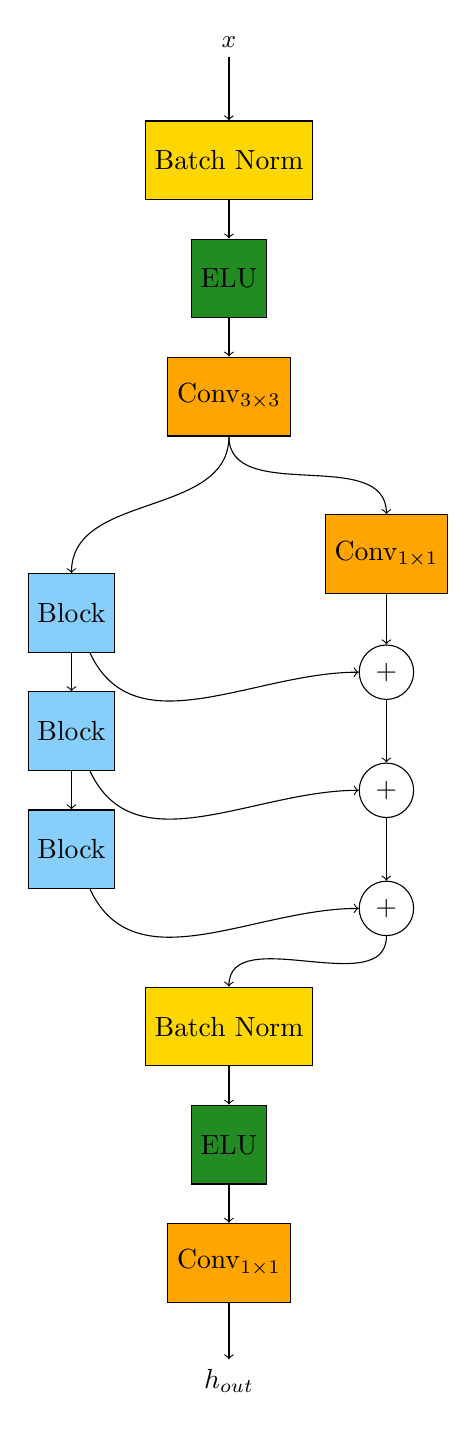
\begin{tikzpicture}
    \node (x) at (0,-1) {\small$x$};
 
    \node[bn] (bn1) at (0, -2.5) {$\text{Batch Norm}$};
    \node[elu] (elu1) at (0, -4) {ELU};
    \node[conv] (conv1) at (0, -5.5) {$\text{Conv}_{3\times3}$};
    \node[conv] (conv2) at (2, -7.5) {$\text{Conv}_{1\times1}$};
    \node[rcb] (rcb1) at (-2, -8.25) {Block};
    \node[circle, draw] (plus1) at (2, -9) {$+$};
    \node[rcb] (rcb2) at (-2, -9.75) {Block};
    \node[circle, draw] (plus2) at (2, -10.5) {$+$};
    \node[rcb] (rcb3) at (-2, -11.25) {Block};
    \node[circle, draw] (plus3) at (2, -12) {$+$};
    \node[bn] (bn2) at (0, -13.5) {$\text{Batch Norm}$};
    \node[elu] (elu2) at (0, -15) {ELU};
    \node[conv] (conv3) at (0, -16.5) {$\text{Conv}_{1\times1}$};
    \node[] (out) at (0, -18) {$h_{out}$};
    
    \draw[->] (x) to (bn1);
    \draw[->] (bn1) to (elu1);
    \draw[->] (elu1) to (conv1);
    \draw[->,out=270, in=90] (conv1) to (conv2);
    \draw[->, out=270, in=90] (conv1) to (rcb1);
    \draw[->] (rcb1) to (rcb2);
    \draw[->, out=295, in=180] (rcb1) to (plus1);
    \draw[->] (conv2) to (plus1);
    \draw[->] (rcb2) to (rcb3);
    \draw[->, out=295, in=180] (rcb2) to (plus2);
    \draw[->] (plus1) to (plus2);
    \draw[->, out=295, in=180] (rcb3) to (plus3);
    \draw[->] (plus2) to (plus3);
    \draw[->, out=270, in=90] (plus3) to (bn2);
    \draw[->] (bn2) to (elu2);
    \draw[->] (elu2) to (conv3);
    \draw[->] (conv3) to (out);
\end{tikzpicture}
\end{document}